\documentclass[a4paper,pdf,12pt]{article}

\usepackage[utf8]{inputenc}

\usepackage{algorithmic}
\usepackage{amssymb}
\usepackage{tikz}

\usepackage{comment}
\usepackage{amsmath}
\usepackage{mathtools}
\usepackage{multirow}

\usepackage{natbib}

\usepackage{graphicx}
\usepackage{array}

\usepackage{caption}
\usepackage{subcaption}

\usepackage{rotating}

\usepackage[english]{babel}

\usepackage{url}
\usepackage[a4paper=true]{hyperref}
\hypersetup{
    colorlinks=false,
    pdfborder={0 0 0},
}


\title{Crowd Manipulation Game\\ \normalsize{Game Programming}}
\author{Steven Laan\\UvAnetID: 6036031\\\url{S.Laan@uva.nl} \and Michael Cabot\\UvAnetID: 6047262\\\url{Michael.A.Cabot@gmail.com} \and Richard Rozeboom\\UvAnetID: 6173292\\\url{HyperSqual@gmail.com}}
\date{\today}

\begin{document}

\maketitle
\abstract{This report describes how a top-down game can be made using the Python toolkit Pygame. The game's focus will be on crowd simulation and manipulation, using methods such as Astar and steering behavior. The game, dubbed Crowd Manipulation Game, features two levels to solve, and includes a level editor for further use}

\section{Introduction}
% TODO background / motivation
Crowd behavior has been of great interest in the field of Artificial Intelligence tackling the problem of simulating large amounts of people. Every individual in a group of people has to take  many decisions when navigating through the crowd. People would rather not bump into each other, and will try to leave some space between one another. As each person will have a certain place to be, they will not stand still to avoid bumping into each other but instead will try to steer around each other. This requires estimating when and how much to turn, what speed to move at, and calculating an optimal path to the current destination. In crowd simulation these decisions and estimations have to be made for each individual agent.
%http://www.youtube.com/watch?v=eGYIEvEe7Ks

Crowd manipulation is the intentional use of techniques to control or influence the behavior of a crowd such that they take upon a desired action. In the Crowd Manipulation Game (CMG) the player is equipped with artifacts and special abilities which allows him to manipulate the crowd such that he is able to achieve a desired goal. The game is somewhat inspired by the upcoming game Watchdogs\citep{watchdogs}, where the player can manipulate the environment by hacking devices such as cell phones and stoplights. In CMG the player will be able to `hack' ATM machines, making them spit out money in the environment, and civilians will be eager to pick this money up.

% TODO explain pygame
The game is made using the open source Pygame toolkit\footnote{\url{http://www.pygame.org}}: a set of Python modules designed for writing games. Pygame allows the use of functions that are typically used in the making of games, such as support for sprites, collision, rendering and the likes. 

Section \ref{sec:Design} will discuss the graphical design of the CMG and section \ref{sec:Rendering} will discuss how all the visuals are rendered. In section \ref{sec:Collision Detection} our collision detection is detailed. Section \ref{sec:Path Planning} discusses two approaches to path planning and section \ref{sec:Steering Behavior} explains two approaches to steering behavior. Section \ref{sec:Gameplay} gives an overview of the current state of the game and sections \ref{sec:Discussion} and \ref{sec:Future Work} discuss possible adjustments and extensions. Finally, section \ref{sec:Conclusion} concludes our work.

\section{Design}
\label{sec:Design}
% TODO pixal art, \ref{fig:player}

Our game engine consist of several classes and a main loop. Our structure allows for an easy object oriented extension. 

The primary class for the objects in the game is the GameObject class. Every object in the game should be a subclass of GameObject. 

The engine keeps track of a list of GameObjects. It also has an Level instance. The Level object contains the information for one level. Things such as what GameObjects should be created where and the locations of walls are stored in the Level class. The Level class also contains code for collision checking and moving around as will be discussed in more detail in sections \ref{sec:Collision Detection} and \ref{sec:Path Planning}.

The main loop dispatches a slice of computation time to each object, so that it can perform its logic. After each GameObject has had their slice, everything is drawn to the screen.

\section{Rendering}
\label{sec:Rendering}

\begin{figure}
        \centering
        \begin{subfigure}[b]{0.4\textwidth}
                \centering
                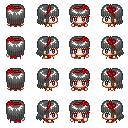
\includegraphics{../img/player.png}
                \caption{Player sprites.}
                \label{fig:player}
        \end{subfigure}%
        ~ %add desired spacing between images, e. g. ~, \quad, \qquad etc.
          %(or a blank line to force the subfigure onto a new line)
        \begin{subfigure}[b]{0.4\textwidth}
                \centering
                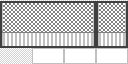
\includegraphics{../img/ground_test.png}
                \caption{Wall tileset.}
                \label{fig:walls}
        \end{subfigure}
        \caption{Some sprites}\label{fig:sprites}
\end{figure}

In simple top-down games you can draw almost in arbitrary order. However, because we use a bird-view perspective, care has to be taken when drawing things. Some objects obscure other objects and therefore have to be drawn after the object they are obstructing. Our renderer takes care of this. It sorts all objects based on their depth and draws them in the correct order.

Next to drawing everything in order, our renderer is able to handle tilesets. This way you can use 1 file for all images of one object. See for example the tileset of the player in figure \ref{fig:player}. The renderer selects the right subframe to draw, based on the direction and animation-counter.

For the walls the tileset is shown in figure \ref{fig:walls}. The renderer has a dedicated section for the drawing of static objects, such as walls. Using the tilesets the renderer is able to create seamlessly connected walls.


% TODO tileset

\section{Collision Detection}
\label{sec:Collision Detection}
As soon as the rendering worked, we started on the collision detection, because you don't want your player to be able to walk through walls. Each sprite has a rectangle that represents the boundaries of the object. A collision is detected by determining whether there is an overlap between two rectangles. The overlap between two rectangles is calculated by pygame's \textit{colliderect()}. In some cases it is desirable to inflate the rectangle to detect a collision before the objects actually collide,

An object is able to move in a direction if it does not result in a collision. If the object moves both horizontally and vertically, then the object is only moved in the direction that does not cause a collision. For example, an object that wants to move both upwards and to the right will only move upwards if there is a collision when moving to the right and no collision when moving upwards. This way an object can glide over a wall without the player explicitly having to hold only the valid keys. 

At first every collision was treated in a similar fashion. All objects in the game inherited from a superclass named GameObject, thus making collision detection easy because of polymorphism. However, because there were quite a couple of walls, it also made collision detection a tad slow. Therefore we implemented another system that is quite straightforward: whenever walls lie next to each other merge them to create a bigger rectangle, on which the collisions are tested.

Thus there are 2 collision systems:
\begin{enumerate}
\item One system for GameObjects
\item One system for static wall collisions
\end{enumerate}

\section{Path Planning}
\label{sec:Path Planning}

After we created collision detection, we wanted to implement NPCs, non-playable characters. At first these characters just walked in a straight line. As this is not very smart and does not get you anywhere, more advanced pathplanning had to be implemented. 

\subsection{Grid-based approach}
One of the simplest solutions was to work with the grid we already got for the collisions. Every point in this grid was connected to its direct neighbors in a graph. Now we could simply use A* to plan a path in this graph. 

The planning of a path involved converting the pixel position of an NPC to the corresponding tile position, as this was the level the collision map was defined on. Then the path could be planned in these tile positions and could be executed by the NPCs.

\subsection{Navigation Mesh}
The former solution did work, albeit it was a bit slow. As the goal was to simulate a crowd, slow pathfinding could really become a problem, when dealing with bigger crowds. Thus a more efficient solution had to be found.

Therefore we implemented a navigation mesh for the NPCs to use. By using this mesh instead of all the grid locations, the number of nodes in the planning graph was greatly reduced. In figure \ref{fig:mesh} an example of the navigation mesh can be seen. 

\begin{figure}[h!]
\centering
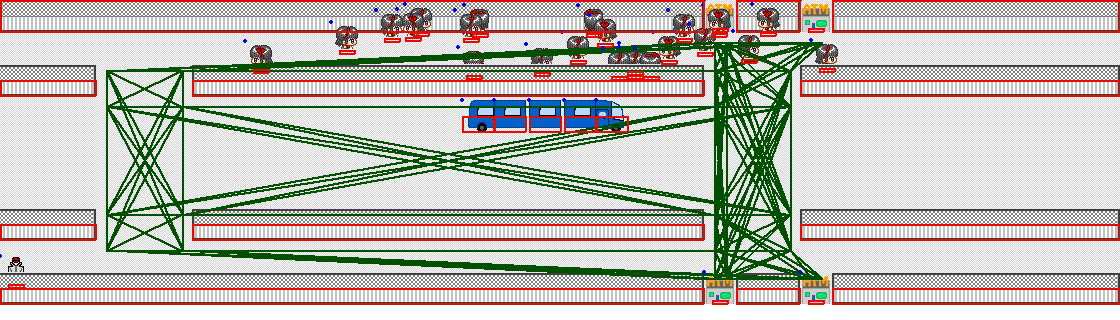
\includegraphics[width = 1.0 \textwidth]{../screenshots/screenshot_16920.png}
\caption{The navigaton mesh is shown in green. The rectangles used for collision detection are shown in red.}
\label{fig:mesh}
\end{figure}

\section{Steering Behavior}
\label{sec:Steering Behavior}

The pathfinding plans a path around the static walls in the level. There are however a couple of dynamic objects in our world as well, e.g. the player and NPCs. Instead of making the pathplanning significantly more difficult, we use steering behaviors to avoid the dynamic obstacles. 

\subsection{Boids approach}
The first thing we tried was to implement a similar system to the Boids that were discussed in \citep{reynolds1987flocks}. The individuals were able to keep their distance, but it looked rather unnatural. Another problem with this approach was that sometimes one individual would push another away from its goal, while that other individual was pushing him. Thus both never reached their goals.

Because this did not work out as we planned we tried another approach.

\subsection{Scanline approach}
The scanline approach employs ray casting to guide steering. Basically each person shoots three rays: 1 straight ahead, 1 tilted to the left and 1 tilted to the right, forming an arc in front of the agent. Based on which lines are triggered, the heading direction is altered, such that the detected entity is being avoided, while still heading towards the destination. When an entity is touched by one of the lines, the turning angle increases incrementally to a certain amount. When the entity is no longer in the cone of the agent, the turning angle gradually decreases until it is back to no turning at all. This will make agents make a curve around other agents, mimicking human steering behavior.

\section{Gameplay}
\label{sec:Gameplay}
Figure \ref{fig:gameplay} shows some typical gameplay. A bus appears on the left side of the screen heading west and lots of people are standing near the northern ATMs. The player, located in the bottom right corner of the screen, has to try and catch the bus before is leaves the screen. When dropping money on the street, people will try to pick thus blocking the road for the bus. This allows the player to get on the bus and drive off once the money is gone and the people walk away.

\begin{figure}
        \centering
        \begin{subfigure}[b]{0.4\textwidth}
                \centering
                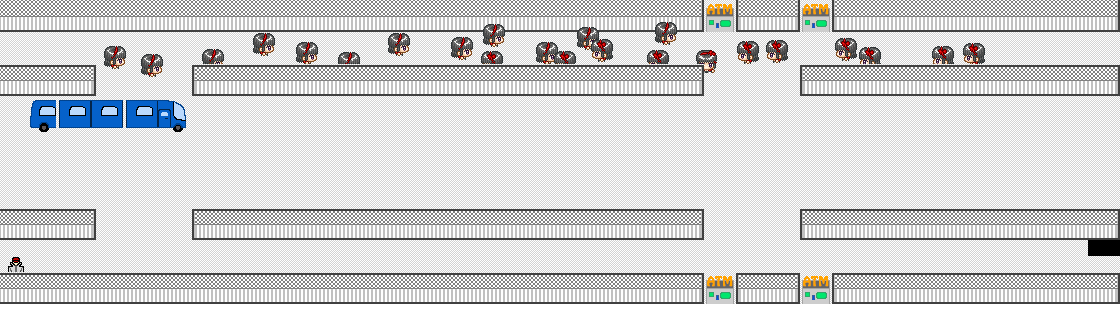
\includegraphics[width=\textwidth]{../screenshots/screenshot_5336.png}
                \caption{Start of the game.}
                \label{fig:screenshot01}
        \end{subfigure}%
        ~ %add desired spacing between images, e. g. ~, \quad, \qquad etc.
          %(or a blank line to force the subfigure onto a new line)
        \begin{subfigure}[b]{0.4\textwidth}
                \centering
                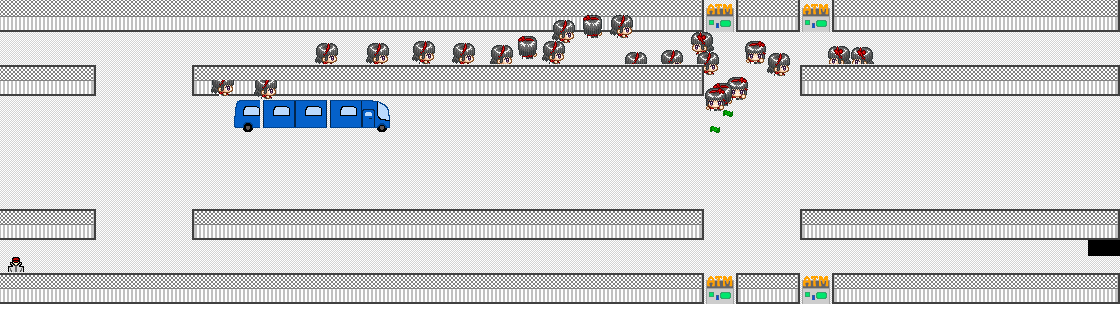
\includegraphics[width=\textwidth]{../screenshots/screenshot_9475.png}
                \caption{Drop some money.}
                \label{fig:screenshot02}
        \end{subfigure}

        %add desired spacing between images, e. g. ~, \quad, \qquad etc.
          %(or a blank line to force the subfigure onto a new line)
        \begin{subfigure}[b]{0.4\textwidth}
                \centering
                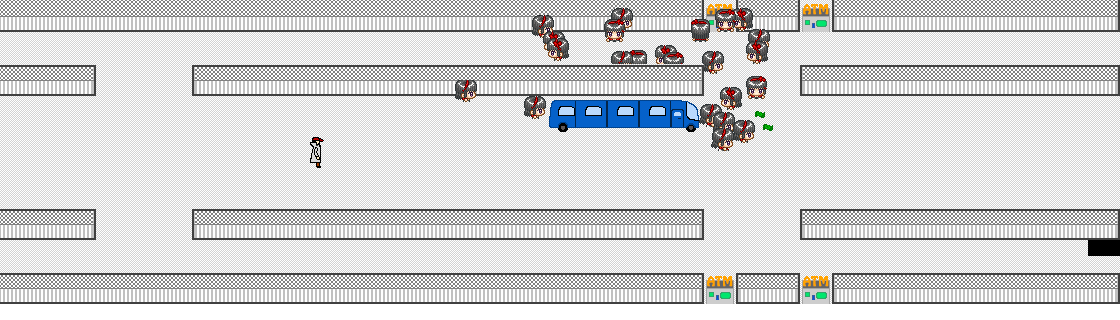
\includegraphics[width=\textwidth]{../screenshots/screenshot_18178.png}
                \caption{People gain interest.}
                \label{fig:screenshot03}
        \end{subfigure}
        ~ %add desired spacing between images, e. g. ~, \quad, \qquad etc.
          %(or a blank line to force the subfigure onto a new line)
        \begin{subfigure}[b]{0.4\textwidth}
                \centering
                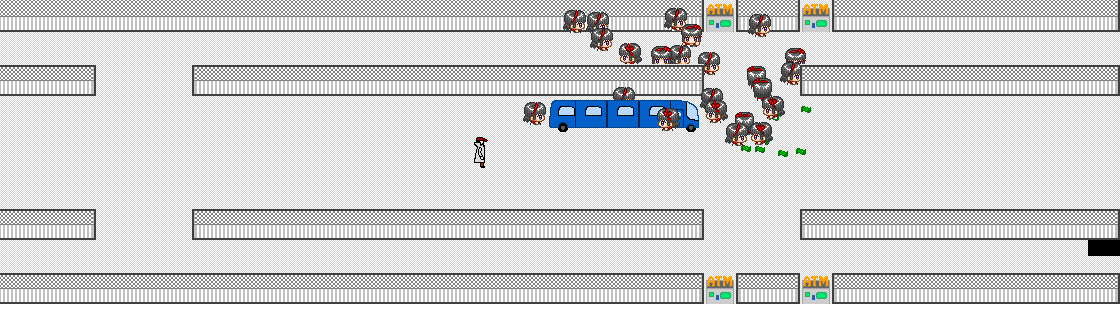
\includegraphics[width=\textwidth]{../screenshots/screenshot_23227.png}
                \caption{Drop some more money!}
                \label{fig:screenshot04}
        \end{subfigure}
        %add desired spacing between images, e. g. ~, \quad, \qquad etc.
          %(or a blank line to force the subfigure onto a new line)

        \begin{subfigure}[b]{0.4\textwidth}
                \centering
                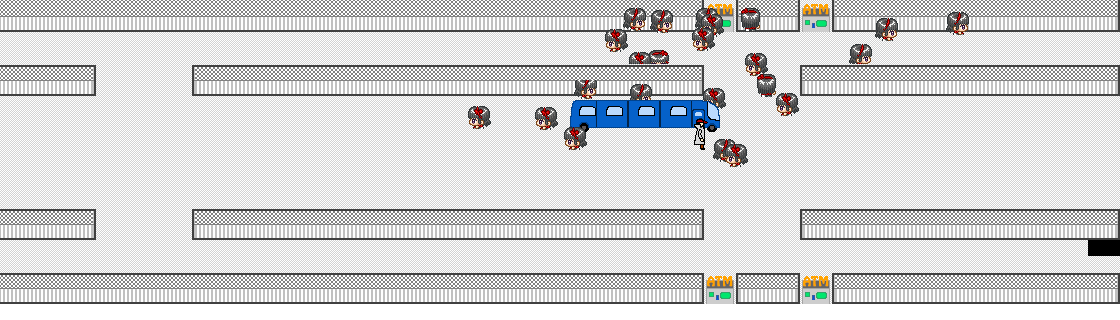
\includegraphics[width=\textwidth]{../screenshots/screenshot_31108.png}
                \caption{Get inside the bus and wait for people to leave.}
                \label{fig:screenshot05}
        \end{subfigure}
        ~ %add desired spacing between images, e. g. ~, \quad, \qquad etc.
          %(or a blank line to force the subfigure onto a new line)
        \begin{subfigure}[b]{0.4\textwidth}
                \centering
                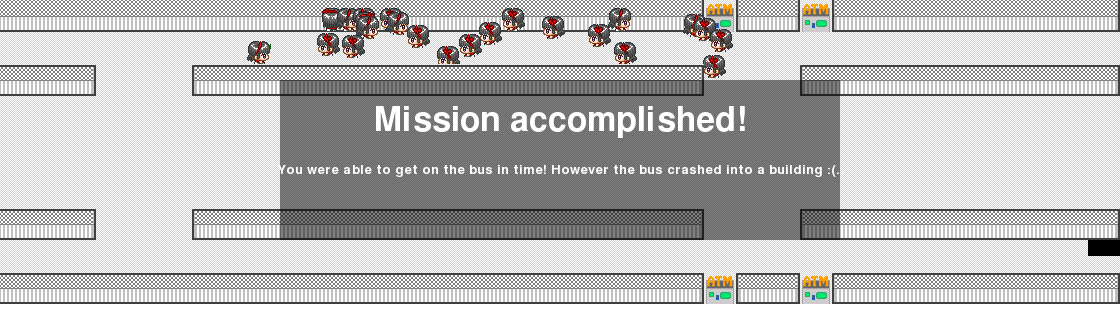
\includegraphics[width=\textwidth]{../screenshots/screenshot_62502.png}
                \caption{End of the level.}
                \label{fig:screenshot06}
        \end{subfigure}

        \caption{Typical gameplay}\label{fig:gameplay}
\end{figure}

\section{Discussion}
\label{sec:Discussion}
Our steering behavior, which makes use of ray casting, offers a simplistic approach to avoiding collisions between NPCs. This simplicity comes at the cost of being inaccurate and error-prone. For starters, a ray that intersects with an object's rectangle only stores that there was an intersection but not where this intersection occurred. This speeds up the process as the search for intersections can be stopped once one is detected. However, this means that a NPC has no way of differentiation between an object that lies far away and an object that lies nearby. This information could be utilized by conditioning the steering behavior of a NPC of the distance to the intersection. 

Another problem when using ray casting is the coverage. Since we use three rays to detect intersections it is possible for an object to lie exactly between two rays of a NPC and still not be detected. This problem would solved by using an arc to detect the intersection between object. Of course, this would greatly increase the computational costs of the steering behavior.

\section{Future Work}
\label{sec:Future Work}
In future work we plan to add more abilities, more types of NPCs and of course more levels and level elements. Abilities would be made more advanced than they are currently, such as items that attract civilians from a certain distance, or items that will only cause certain types of NPCs to be attracted, such as donuts for the police. An item that repels people can also be a fun game mechanic, such as a stink-bomb or explosions that will make the people run in the opposite direction. Currently the CMG has four types of characters, which we could expand upon. More types of civilians can be added for more variety, such as children, elderly which each will move at different speeds. Furthermore, because we have the level editor, we are able to create more levels relatively easily, however level elements are also needed to create versatile gameplay. For example stoplights which can be `hacked' to create a traffic accident, or commercial screens that can be hacked to the advantage of the player, and other electronic devices such as cellphones, gates, fire alarms.

\section{Conclusion}
\label{sec:Conclusion}

In this rather short period of time, we have created a stable game engine, which can be used to create bird-view perspective games, and includes collision detection for each of the objects. The engine includes a renderer that can cope with depth and overlays. For the NPCs there is a navigation mesh they can use to get around. 

We created an minigame with this engine that tries to model a crowd using steering behaviors, and civilians in the CMG will avoid collision with other agents, much like a human would do. The game features two levels, three types of NPCs and currently one ability for the player to use. If the player fails to complete the second level, he will be terminated and will not get another chance to complete his mission.

The NPCs find their way around the map using the navigation mesh for nodes, and A* to plan a path on these nodes. The civilians avoid collision with each other by using steering behavior which is achieved by altering the angle of the civilian depending on a cone in front of the civilian, making the agents curve around each other.


\bibliographystyle{plainnat}
\bibliography{references}

\end{document}